\begin{frame}{Expected Trade-Off}

\begin{columns}[c,onlytextwidth]

\column{0.55\textwidth}
\centering
\resizebox{\linewidth}{!}{%
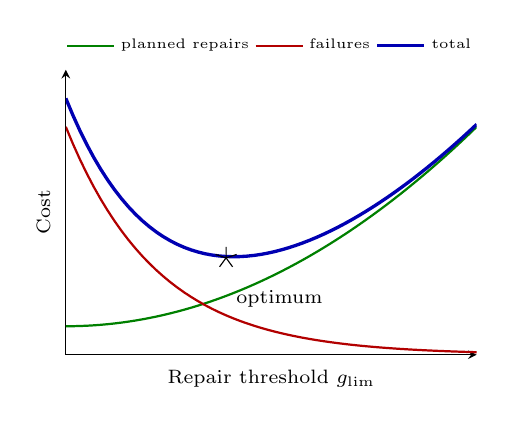
\begin{tikzpicture}
\begin{axis}[
  width=6.8cm, height=5.2cm,
  xlabel={Repair threshold $g_\mathrm{lim}$}, ylabel={Cost},
  xmin=0, xmax=10, ymin=0, ymax=10,
  xtick=\empty, ytick=\empty,
  axis lines=left,
  label style={font=\scriptsize},
  legend style={font=\tiny, at={(0.5,1.02)}, anchor=south, legend columns=3, draw=none},
]
  \addplot[domain=0:10, samples=60, green!50!black, thick] {1 + 0.07*x^2};
  \addplot[domain=0:10, samples=60, red!70!black, thick] {8*exp(-0.45*x)};
  \addplot[domain=0:10, samples=60, blue!70!black, very thick] {1 + 0.07*x^2 + 8*exp(-0.45*x)};
  \legend{planned repairs, failures, total}
  \addplot[only marks, mark=star, mark size=4pt, black] coordinates {(3.9,3.4)};
  \node[font=\scriptsize, anchor=north] at (axis cs:5.2,2.6) {optimum};
\end{axis}
\end{tikzpicture}%
}

{\scriptsize Qualitative sketch (no results yet).}

\column{0.42\textwidth}
\justifying
\begin{itemize}
  \item \textbf{Small $g_\mathrm{lim}$}: few planned repairs, many failures.
  \item \textbf{Large $g_\mathrm{lim}$}: few failures, many planned repairs.
  \item We expect an \textbf{interior optimum}.
  \item The optimum depends on the ratio $c_\mathrm{fail} / c_\mathrm{rep}$.
\end{itemize}

\end{columns}

\end{frame}
